\documentclass{beamer} 
\usepackage[english]{babel}
%\usepackage[utf8x]{inputenc} % acento normal
\usepackage[utf8]{inputenc}
\usepackage{scalefnt}
\usepackage{color, colortbl, multirow}
\usepackage{epstopdf} %usar figura eps
\usepackage{verbatim} % para colocar o comment
%\usepackage[latin1]{inputenc}
\usepackage[algoruled,longend]{algorithm2e}



%\usepackage[applemac]{inputenc} % acento mac

\usepackage{graphicx} % para inserir figuras
%\graphicspath{figuras/} % para caminho da pasta com figuras

\usepackage{adjustbox}

\usepackage{svg}
\usepackage{epsfig}

\setbeamertemplate{navigation symbols}{} % remover barra de navega‹o
\setbeamertemplate{footline}[frame number] % numero de paginas


\usetheme {Frankfurt} %Berlin Malmoe Warsaw Rochester Darmstadt Madrid Antibes Bergen Berkley Boadilla Copenhagen Dresden Frankfurt 
%Goettingen Hannover Ilmenau JuanLesPins Luebeck Marburg Montpellier PaloAlto Pittsburgh Singapore Szeged boxes default CambridgeUS AnnArbor Rochester 

\usecolortheme{seahorse} %dolphin orchid whale
%albatross; beaver; beetle; crane; default; dolphin; dove; fly; lily; orchid; rose;seagull; seahorse; sidebartab; whale; wolverine

\definecolor{light_green}{RGB}{230,255,230} %cria a cor pra ser usada no background
\definecolor{tbGreen}{RGB}{166,210,166}

\setbeamercolor{background canvas}{bg=light_green} % aplica a cor no background
%\useinnertheme{circles} %define os numeradores com o padrão circles
%\setbeamercolor{block title}{fg=white,bg=green!40!black} %define os titulos dos blocos como verde
%\setbeamercolor{itemize item}{fg=green!40!black} %define os marcadores de ítem como verdes
%\setbeamercolor{itemize subitem}{fg=green!40!black} %define os marcadores de sub-ítem como verdes
%\setbeamercolor{item projected}{fg=white,bg=green!40!black} %define os numeradores como verdes

\setbeamercolor{section in toc shaded}{fg=black} %define os links no tableofcontents como preto (quando estão selecionados)
\setbeamercolor{section in toc}{fg=black} %define os links no tableofcontents como preto (quando não estão selecionados)

\setbeamercolor{structure}{bg=black,fg=green!50!black}
%\setbeamercolor{title}{fg=black, bg=green!40!black}
%\setbeamercolor{frametitle}{fg=black, bg=green!80!black}



\pgfdeclareimage[height=1cm]{c-bio}{figuras/c-bio.jpg}
%\logo{\pgfuseimage{c-bio}}
\pgfdeclareimage[height=1cm]{ufpr}{figuras/ufpr.png}
\logo{\pgfuseimage{ufpr} \hspace{276pt} \pgfuseimage{c-bio}}

%%===================== Capa =========================%%

\title{ \textbf{Otimização Multi-objetivo (MOP)} \\ \textbf{Distribuição 
Gaussiana} }

\author{Gian M. Fritsche %\\ \quad \\ \small{Advisor: Prof. Dr. Aurora T. 
% R. Pozo} 
}

\institute{Programa de Pós-Graduação em Informática\\ Universidade Federal do 
Paraná}

\begin{document} % inicio do documento

\date{9 de Março de 2015}

\frame{
	\titlepage
	%\center{\scriptsize{Orientadora: Prof.ª Aurora Trinidad Ramirez Pozo}}

}

\section{Otimização Multi-objetivo}
\subsection{O que é Otimização Multi-objetivo?}

\frame{
	\frametitle{O que é Otimização Multi-objetivo?}
	
	\begin{block}{}
		  \begin{itemize}
		   \item Se refere a otimização simultânea de mais de um 
objetivo.
		  \end{itemize}
	\end{block}

	\vspace{-4pt}
	\hspace{-20pt}
	\begin{minipage}{1.0\textwidth}
		\begin{figure}[ht]
		\centering
			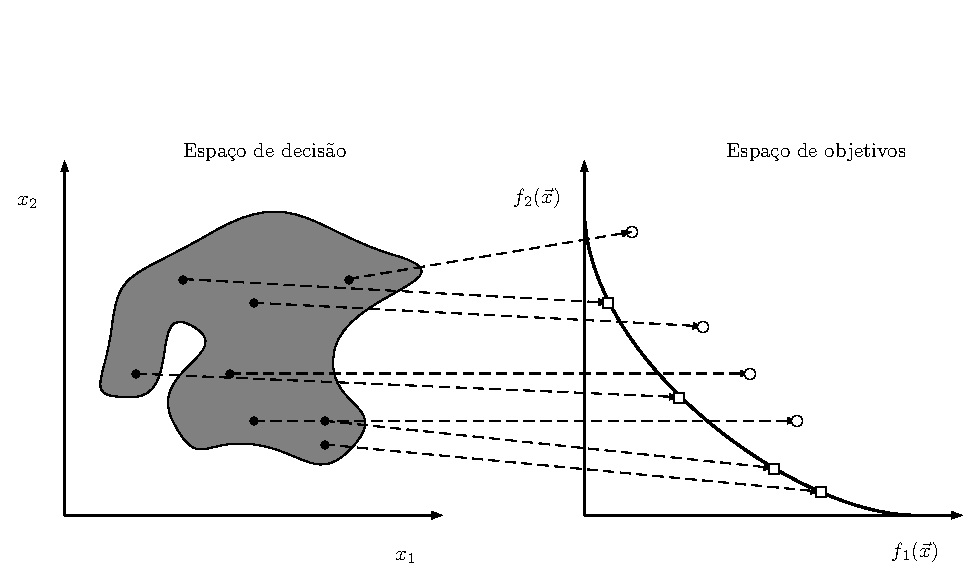
\psfig{file=figuras/pareto.eps,height=6cm}
\caption{Representação de um problema Multi-objetivo}
		      \label{fig:normal-distribution}
		\end{figure}
	\end{minipage}
	
}

\frame{
	\frametitle{Exemplo de problema Multi-objetivo}
	
	\begin{block}{}
		  Olá Mundo.
	\end{block}
}

\frame{
	\frametitle{O que é uma solução em um problema Multi-objetivo?}
	
	\begin{block}{}
		  Olá Mundo.
	\end{block}
}

\section{Distribuição Gaussiana}
\subsection{O que é Distribuição Gaussiana?}
\frame{
	\frametitle{O que é Distribuição Gaussiana?}
	
	\begin{block}{}
	  \begin{itemize}
	    \item  A distribuição Gaussiana ou Normal, é uma curva utilizada 
para calcular a probabilidade de um valor em uma distribuição. 
	    \item Possui apenas 2 parâmetros: média $\mu$ e variância 
$\sigma^2$
	    \item Ou seja, dado um valor de média e variância é possível 
calcular a probabilidade de qualquer valor.
	    \item Uma característica é que a probabilidade dos valores mais 
próximos a média é muito maior do que os valores mais afastados. Cerca de 68\% 
dos valores estão a menos de um desvio padrão da média, 
	  \end{itemize}
	\end{block}
}

\frame{
	\frametitle{Exemplo de distribuição Gaussiana}

	\vspace{-4pt}
	\hspace{-20pt}
	\begin{minipage}{1.0\textwidth}
		\begin{figure}[ht]
		\centering
			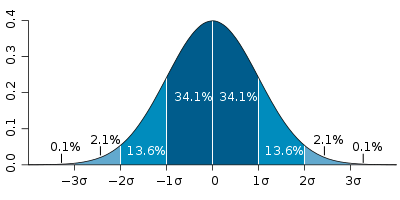
\includegraphics[scale = 
0.5]{figuras/normal-distribution.png}
			\caption{Exemplo de distribuição Gaussiana}
			\label{fig:normal-distribution}
		\end{figure}
	\end{minipage}
	
}

\frame{
	\frametitle{Para que é utilizada a Distribuição Gaussiana?}
	
	\begin{block}{}
		  \begin{itemize}
		   \item Utilizada para prever a probabilidade de um valor em 
um conjunto.
		   \item Diversos conjuntos seguem uma distribuição normal, 
tais como tamanho de produtos produzidos por máquinas, fenômenos naturais e 
financeiros.
		   \item Em geral, a distribuição normal é uma boa aproximação 
de outras distribuições que não tenham as características da distribuição 
normal.
		  \end{itemize}
	\end{block}
}


\frame{
	\frametitle{Qual é a diferença entre distribuição univariada e 
multivariada?}
	
	\begin{minipage}[t]{0.45\linewidth}
\centering
\begin{block}{} 
	      \begin{itemize}
	       \item A distribuição normal multivariada é uma distribuição 
normal com mais de uma variável.
	      \item Utilizada para descrever aproximadamente a relação entre as 
variáveis.
	      \end{itemize}
\end{block}
\end{minipage}
\hspace{0.5cm}
\begin{minipage}[t]{0.45\linewidth}

\begin{figure}
	\centering
	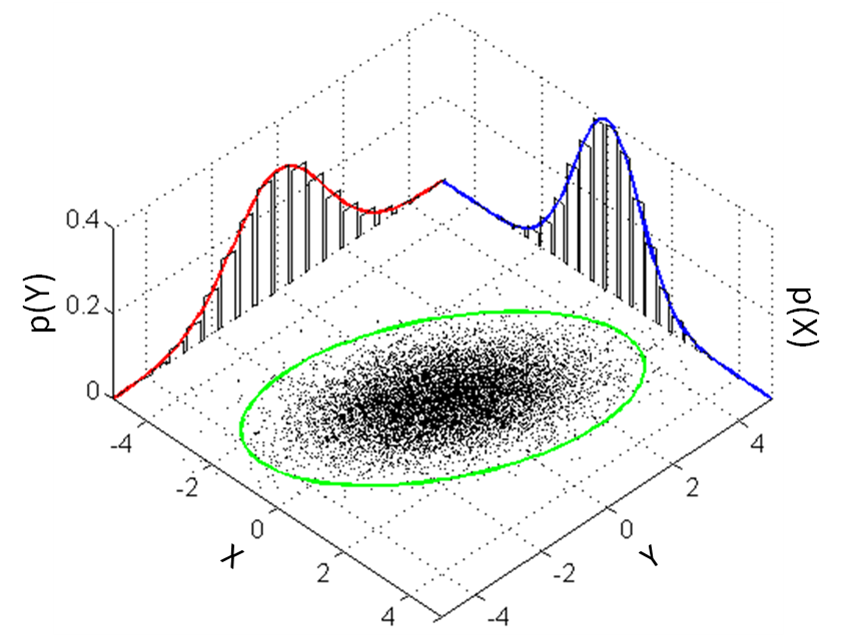
\includegraphics[width= 2 in] {figuras/multivariate-normal.png}
	\end{figure}
\end{minipage}

}

\frame{
	\frametitle{}
 
	\begin{block}{}
		\centering Obrigado! \\ \quad \\ \quad \\
		\centering Gian Mauricio Fritsche \\
		\centering \small gmfritsche@inf.ufpr.br
	\end{block}

}	

\end{document} 


